\documentclass[11pt]{beamer}
\usepackage{helvet} %font
\beamertemplatenavigationsymbolsempty
\usetheme{JuanLesPins}
\usefonttheme{structurebold}

\usepackage[french]{babel}
\usepackage[utf8]{inputenc}
\usepackage[T1]{fontenc}
\usepackage{amssymb,amsmath}
\usepackage{tikz}
\usepackage{geometry}
\usepackage{xcolor,colortbl}
\usetikzlibrary{arrows,positioning}
\usepackage{listings}

\AtBeginSubsection[]
{
   \begin{frame}
	\small \tableofcontents[currentsection]
   \end{frame}
}

\newenvironment{slide}[1]{%
\begin{frame}[environment=slide]
\frametitle{#1}
}{%
\end{frame}
}
\setbeamercolor{structure}{fg=red}
\setbeamercolor{frametitle}{bg=black,fg=white}
\definecolor{gris}{gray}{0.6}
\definecolor{grisclair}{gray}{0.9}

\newtheorem{exercice}{Exercice}

\title{Machine Learning IV \\ Classification non supervisée}
\author{Nicolas Bourgeois}
\date{}

\newcommand{\Python}[1]{
	{\small	\lstinputlisting[language=Python]{./#1.py}}
}
\newenvironment{pyenvsmall}
	{ \ttfamily \tiny }
	{\par  }

\newcommand{\Pythonsmall}[1]{
	{\scriptsize \lstinputlisting[language=Python]{./#1.py}}
}
\newcommand{\elimine}[1]{{\textcolor{lightgray}{#1}}}

\newcommand\Wider[2][3em]{%
\makebox[\linewidth][c]{%
  \begin{minipage}{\dimexpr\textwidth+#1\relax}
  \raggedright#2
  \end{minipage}%
  }%
}

\begin{document}

\begin{frame}
\maketitle
\end{frame}

\begin{frame}{K-means : objectif}

On dispose de n données et de p variables.\\

\pause
\vspace{0.2cm}

On veut créer une partition qui minimise la somme des inerties internes à chaque classe.\\

$$\min \sum_{i \leq k} \sum_{x \in Z_i} d^2(x,\bar{z}_i)$$
où $\bar{z_i}$ est le centre de $Z_i$.

\end{frame}

\begin{frame}{K-means : base}

On initialise les centres aléatoirement, puis à chaque étape :
\pause
\begin{itemize}
	\item On affecte chaque donnée au centre le plus proche
	\item On recalcule la position des centres
\end{itemize}

\end{frame}


\begin{frame}{Exercice}

\begin{exercice}
Importez les données iris avec \texttt{dataset.load\_iris}. Effectuez un k-means avec 2,3,4 valeurs. Comparez graphiquement les résultats avec les valeurs cibles.
\end{exercice}

Attention : L'objectif ici n'est pas de prédire Y, mais de mettre en correspondance Y avec un clustering ne dépendant que de X.

\end{frame}

\begin{frame}{Résultat attendu}
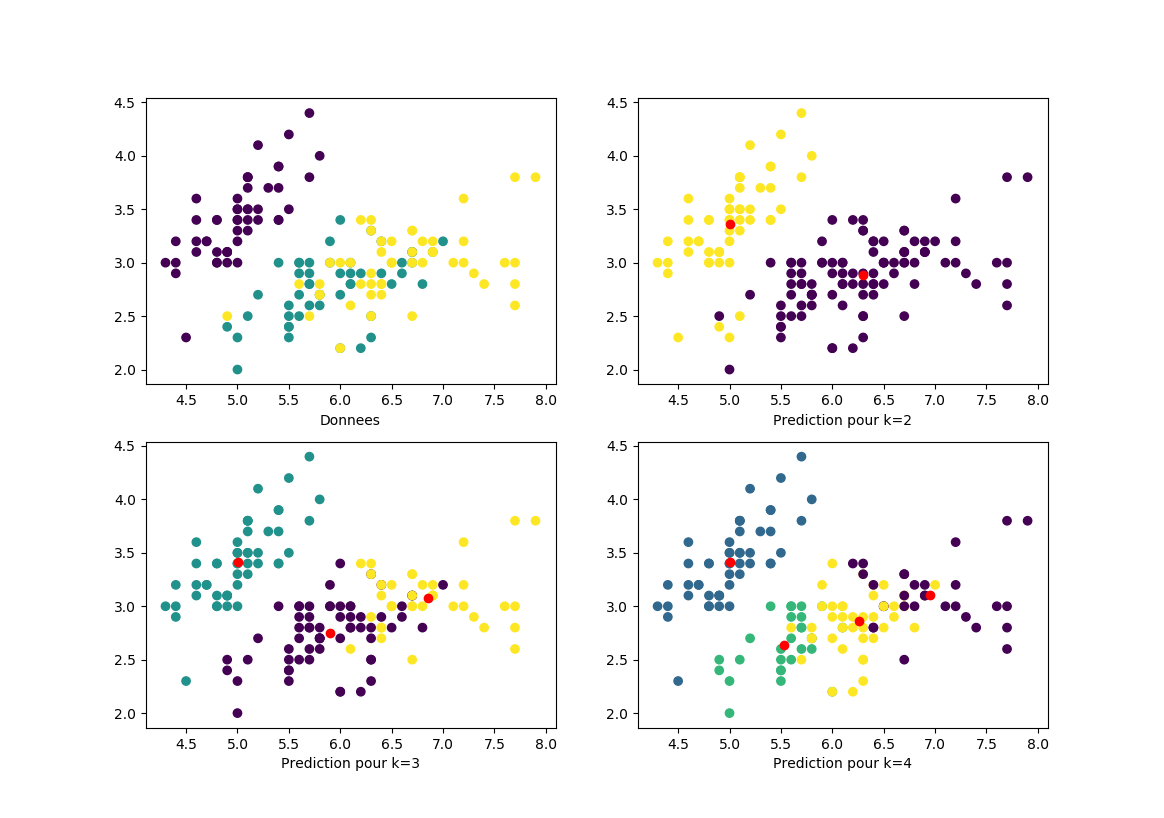
\includegraphics[scale=0.35]{ex501}
\end{frame}

\begin{frame}{Solution}
\Pythonsmall{ex501}
\end{frame}


\begin{frame}{Exercice}

\begin{exercice}
Séparez maintenant vos données en un échantillon d'apprentissage et un échantillon de test. Visualisez (par exemple avec des différences d'opacité) dans quels clusters sont placées les nouvelles valeurs.
\end{exercice}

\end{frame}

\begin{frame}{Résultat attendu}
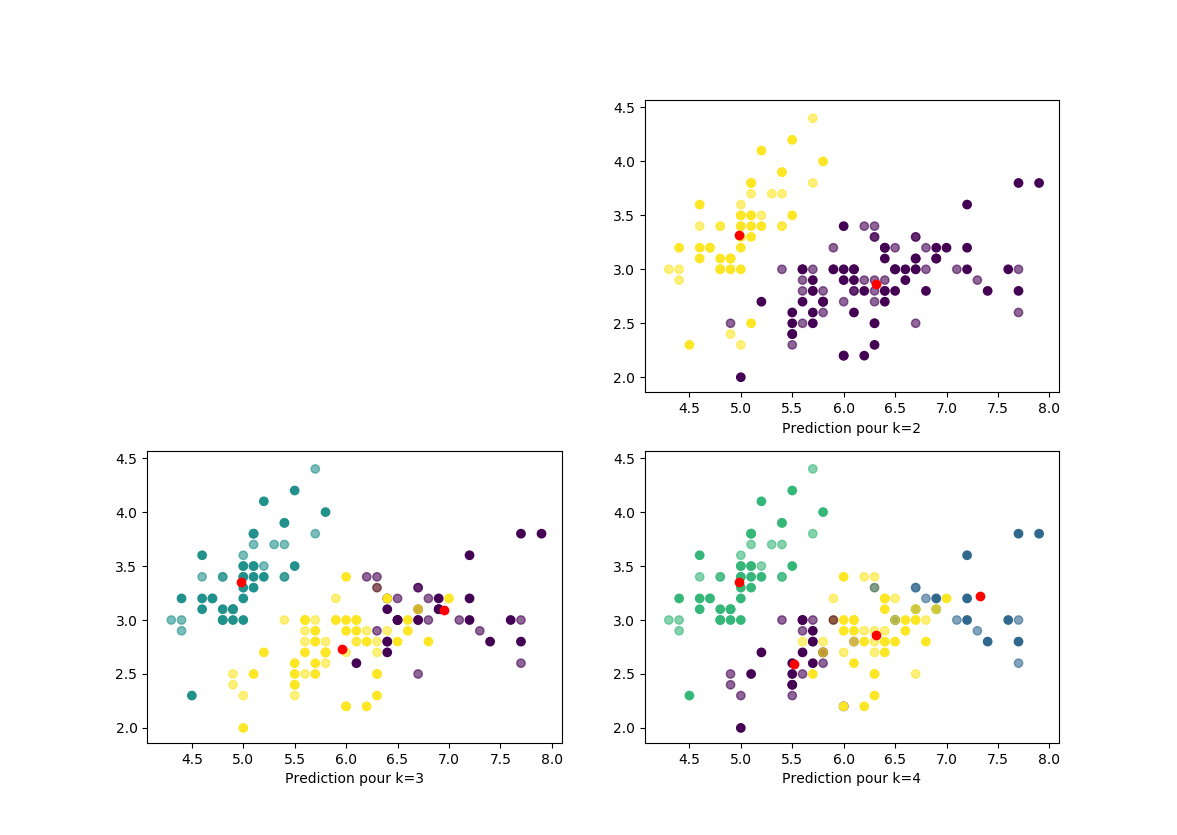
\includegraphics[scale=0.35]{ex501bis}
\end{frame}

\begin{frame}{Solution}
\Pythonsmall{ex501bis}
\end{frame}


\begin{frame}{Problèmes}

\begin{itemize}
	\item Pas de garantie d'optimalité
	\item Pas de garantie de polynomialité (par rapport à n)
	\item Choisir k a priori
\end{itemize}

\end{frame}

%%%%%%%%%%%%%%%%%%%%%%%%%%%%%%%%%%%%

\end{document}

